
\chapter{MEDICIÓN Y DEMOSTRACIÓN DE RESULTADOS EXPERIMENTALES.}

\section{A través de medios electrónicos o mecánicos, de al menos los puntos b), c) y d).
}

\subsection{Sensor de proximidad}
\href{https://youtu.be/l9V6qCGNVYA}{En este video } \textrm{: se puede apreciar un demo de cómo mediremos la deformación de la viga.}
\bigskip
\bigskip
\begin{center}
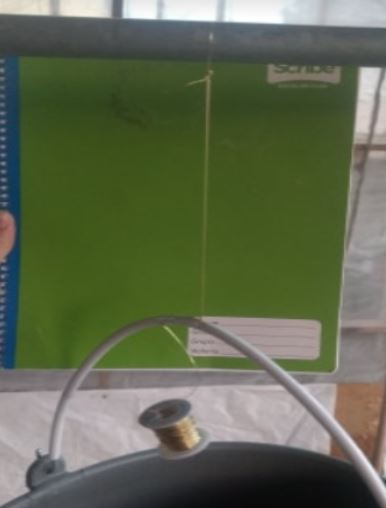
\includegraphics[width=.8\linewidth]{E/figs/A_1.jpg} 
\end{center}
\bigskip
\bigskip
\bigskip
\bigskip
\bigskip

\subsection{Bot telegram}
\textrm{ De ser posible también tendremos un Bot que nos dará las métricas de todos los puntos solicitados}

\begin{center}
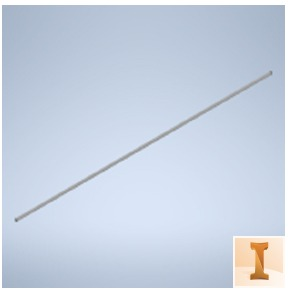
\includegraphics[width=.6\linewidth]{E/figs/A_2.jpg} 
\end{center}